\documentclass[11pt]{beamer}
\usetheme{fdu}

%%% Packages
\usepackage{ulem}  % 导言区加载
\usepackage{tikz} % plot in place
\usepackage{pgfplots} % rather include jpg/pdf
\pgfplotsset{compat=1.9}
\usepackage{diagbox} % diagbox for table
\usepackage[export]{adjustbox} % autofix for table
\usepackage[ruled]{algorithm2e}
\SetAlCapFnt{\tiny\sffamily} % setting fonts for algorithm caption
\usepackage[round]{natbib} % bib cite package
\usepackage{xcolor}
\bibliographystyle{dinat} % set bib style
\setbeamercovered{transparent} % shadow words for overlay

\usepackage{subcaption}
\usepackage{graphicx}


\usepackage{booktabs}
\usepackage{array} 

\usepackage{listings}

\usepackage{fontspec}
\usepackage{xeCJK} % CJK package for xelatex
% \setCJKmainfont{SimHei} % use SimHei as main font <- need preinstall SimHei
%\setbeamertemplate{caption}[numbered] % add caption number for figure and table
\setmainfont{Times New Roman}
\setCJKmainfont{STSong}

%%% Titlepage information
\title[2025年春季统计软件课程项目]{胸腔 CT 图像二分类问题}
\author[Presenter isKage]{isKage \and Author2 \and Author3}
\institute[复旦大学]{
    复旦大学管理学院 \\
    School of Management, Fudan University, Shanghai, China\\[0.5cm]
    \tiny{本项目已开源在 Github 地址 \href{https://github.com/isKage/r-course-pj}{https://github.com/isKage/r-course-pj}\\[0.4em]
    拓展:卷积神经网络代码已开源在 Kaggle 地址 \href{https://www.kaggle.com/code/iskage/ct-images-cnn/}{https://www.kaggle.com/code/iskage/ct-images-cnn/}}
}

% table of contents
\AtBeginSection[]{
    \begin{frame}<beamer>{Agenda}
    \tableofcontents[
        currentsection,
        currentsubsection, 
        hideothersubsections, 
        sectionstyle=show/shaded,
    ]
    \end{frame}
}

\begin{document}

\begin{frame}
  \titlepage
\end{frame}

\begin{frame}{概述}{}
\fontsize{9pt}{11pt}\selectfont
CT-Images 数据集包括 $1500$ 张正常胸腔 CT 截面图,$1500$ 张患癌胸腔 CT 截面图。
项目目标是实现“正常-患癌”二分类问题,并对 CT 图片进行特征提取,以期获得更精确的医学诊断和解释,
为以后的研究提供统计推断的依据。\\[0.5em]

主要使用的方法包括:主成分分析法(PCA)、Logistic 回归、聚类分析、卷积神经网络。
\begin{itemize}
  \item 主成分分析用于图像降维(作为拓展,尝试使用 MaxPool 最大池化方法进行降维)
  \item 聚类分析用于初步分析
  \item Logistic 回归用于二分类
  \item 卷积神经用于更为精细的二分类
\end{itemize}
\end{frame}


\section{数据描述}
\begin{frame}{数据描述}{}
\fontsize{9pt}{11pt}\selectfont

拟研究的问题:CI-Images 肺部 CT 图的“正常-患癌”二分类问题。
CT-Images 数据集包括 $1500$ 张正常肺部 CT 图,$1500$ 张患癌肺部 CT 图,(数据平衡性满足)。\\[0.5em]

其中每一个 CT 图已经过处理,为 \texttt{.jpg} 格式,具有 RGB 三通道。但都经过了黑白化处理,
可以转换为 \texttt{.png} 单通道格式读入程序(tips: 图片像素点在处理后值仅为 $0$ 和 $1$)。

\begin{figure}
  \centering
  
\includegraphics[width=0.3\linewidth]{../assets/normal.jpg}
  \hspace{0.05\linewidth}
  
\includegraphics[width=0.3\linewidth]{../assets/cancer.jpg}
  \caption{左图:正常 CT 图;右图:患癌 CT 图}
\end{figure}

\end{frame}


\section{图像处理}
\begin{frame}{图像处理}{}
\fontsize{9pt}{11pt}\selectfont

图像数据可以理解为一个 $3$ 维张量,分别为 $(H,\ W,\ C)$ 
其中 $H,\ W$ 分别表示图片的长和宽,而 $C$ 代表了图片的通道数
(例如 $C = 1$ 则为单通道灰度图,$C = 3$ 则为常见的 RGB 三通道图片)。\\[0.5em]

在本项目中,我们先读取图片,得到 $H \times W \times C$ 的张量,
经处理得到灰度图,即为 $H \times W$ 的矩阵,每个元素的数值代表像素值。
将图片矩阵展平,得到一个图片向量 $v \in \mathbb{R}^{HW}$ 。
本项目将图片统一为 $p = 224 \times 224$ 维度的向量 $v \in \mathbb{R}^p$ 。

$$
v \in \mathbb{R}^p
$$

如此将 $n$ 个样本读入程序,按行合并成为一个样本矩阵 $X \in \mathbb{R}^{n \times p}$ 
其中每一行代表一个图像样本向量,每一列代表某一位置的像素值。

$$
X \in \mathbb{R}^{n \times p}
$$

\end{frame}



\section{数据降维}

\begin{frame}{PCA 主成分分析}{}
\fontsize{9pt}{11pt}\selectfont

由于原来的样本数据向量 $x \in \mathbb{R}^p,\quad p = 224\times 224 = 50176$ ,
特征维度过高,难以进行分析和建模,故可以采用\textcolor{red}{主成分分析 PCA 方法}进行降维。\\[0.5em]

主成分分析(Principal Component Analysis, PCA)
由 Hotelling 于 1933 年首先提出\citep*{hotelling1933pca}。 
目的是把多个变量压缩为少数几个综合指标(称为主成分),使得综合指标能够包含原来的多个变量的主要的信息。
下面以总体主成分为例,进行算法推导:\\[0.5em]

对于我们这个问题的每一个样本,在被抽样前均为随机变量 $\widetilde{X} \in \mathbb{R}^p$ ,
设其协方差存在且为 $\Sigma \in \mathbb{R}^{p \times p}$ ,对协方差进行谱分解得到:

$$
\Sigma = P \Lambda P^T
$$

其中 $P \in \mathbb{R}^{p\times p}$ 为正交阵,
而 $\Lambda \in \mathbb{R}^{p \times p}$ 为对角阵,且对角元素为 $\Sigma$ 的特征值,即 $\Lambda = diag(\lambda_1,\ \lambda_2,\ \cdots,\ \lambda_p)$ ,且特证值按降序排列 $\lambda_{i} \geq \lambda_{i+1}$ 。


\end{frame}


\begin{frame}{PCA 主成分分析}{}
\fontsize{9pt}{11pt}\selectfont
设 $p_j$ 为第 $j$ 个的特征向量,即 $P$ 的第 $j$ 列。则有 $\widetilde{X}$ 的第 $j$ 个主成分:

$$
Y_j = p_j^T \widetilde{X}
$$

记 $Y = \left[Y_1,\ Y_2,\ \cdots,\ Y_p\right] = P^T \widetilde{X} \in \mathbb{R}^p$ ,则有:

$$
Cov(Y) = Cov(P^T X) = P^T Cov(\widetilde{X}) P = P^T \Sigma P = P^TP\Lambda P^TP = \Lambda
$$

如上构造的主成分 $Y_j$ 为 $\widetilde{X}$ 的线性组合,
且满足在 
$$
Y_j \perp Y_k,\quad k = 1,\ 2,\ \cdots,\ j-1
$$

使得 $Var(Y_j)$ 最大的线性组合,直观地理解就是 $\widetilde{X}$ 在 $Y_j$ 
方向上被尽可能的分开(方差尽可能大)。\\[0.5em]

在本问题中,为实现降维,可以选择这 $p$ 个主成分的前 $q$ 个,
即由原来样本 $x \in \mathbb{R}^p$ 降低到 $x' \in \mathbb{R}^q$ 。

\end{frame}


\begin{frame}{PCA 主成分分析}{}
\fontsize{9pt}{11pt}\selectfont

但这仍然存在问题,即数据维度 $p = 50176$ 远远大于样本量 $n = 3000$ ,同时我们也无法获得一个五万级别大小的矩阵的谱分解,
所以下面提出一种更新的方法,借由\textcolor{red}{矩阵奇异值分解(SVD 分解)}的思想计算。\\[0.5em]

如果我们已经获取到了样本信息,构造出了样本矩阵 $X \in \mathbb{R}^{n\times p}$ ,
假设 $X$ 已经中心化,即 $\bar{X} = \bf{0} \in \mathbb{R}^p$ 。
我们的目标是找到一组正交的向量 

$$
v_1,\ v_2,\ \cdots,\ v_p \in \mathbb{R}^p
$$

将数据投影到这些方向上后,使得投影后的数据具有最大的方差,即:

$$
\max_{v_j \perp v_1,\ v_2,\ \cdots,\ v_{j-1}} Var(Xv_j) = \frac{1}{n} \frac{\|Xv_j\|^2}{\|v_j\|^2} = \frac{1}{n} \frac{v_j^T X^T X v_j}{v_j^Tv_j}
$$

\end{frame}

\begin{frame}{PCA 主成分分析}{}
\fontsize{9pt}{11pt}\selectfont

由\uline{引理 1} :正定阵 $A$ 第 $j$ 个特征值和特征向量为 $(\lambda_i,\ e_i),\quad \lambda_i \geq \lambda_{i+1}$ 则有

$$
\max_{x \perp e_1,\ e_2,\ \cdots,\ e_{j-1}} \frac{x^TAx}{x^Tx} = \lambda_j,\quad \text{when}\ \ x = e_{k}
$$

可知原问题最优解 $v_j^*$ 为 $X^TX$ 的第 $j$ 个特征向量。于是我们对 $X$ 进行 SVD 分解:

$$
X = U \Lambda V^T
$$

其中 $U \in \mathbb{R}^{n\times n},\ V \in \mathbb{R}^{p \times p}$ 
且满足 $UU^T = I_n,\ VV^T = I_p$ 。而 $\Lambda \in \mathbb{R}^{n \times p}$ 为
对角矩阵,主对角线为降序排列的奇异值,其他位置为零。

\end{frame}


\begin{frame}{PCA 主成分分析}{}
\fontsize{9pt}{11pt}\selectfont
注意到:

$$
X^TX = V\Lambda^T U^TU\Lambda V^T = V\Lambda^T \Lambda V^T
$$

其中 $X^TX,\ \Lambda^T\Lambda,\ V \in \mathbb{R}^{p\times p}$ ,
完全符合谱分解的形式,故 $V$ 的每一列均为 $X^TX$ 的特征向量,
即这里的 $V$ 的每一列就是我们要找的最优 $v_j^*$ ,下面介绍如何更高效的求解 $X^TX$ 的特征向量。\\[0.5em]

若记 $u \in \mathbb{R}^n$ 为 $XX^T \in \mathbb{R}^{n\times n}$ 的特征向量,
特征值为 $w$ ,则有 $XX^T u = wu$ ,左乘 $X^T$ 有:

$$
X^TXX^Tu = (X^TX) \cdot X^Tu = X^T wu = w \cdot (X^Tu)
$$

故有 $X^Tu$ 为 $X^TX$ 的特征向量。
所以我们可以通过求解 $XX^T$ 的特征向量 $u$ 进而推出 $X^TX$ 的特征向量 $v = X^Tu$ 。
需要注意的是,$XX^T \in \mathbb{R}^{n \times n}$ 维度为 $n$ ,
当样本量远小于特征量 $p$ 时(例如本问题),采用这个方法能极大的提高计算效率。同样地,为了降维,我们只需选取 $XX^T$ 的前 $q$ 个特征向量即可。

\end{frame}


\begin{frame}{PCA 主成分分析}{}
\fontsize{9pt}{11pt}\selectfont

虽然上面的方法已经极大地节约了计算成本,但当遇见 $n$ 样本量同样巨大的问题
(例如本问题),求解 $XX^T \in \mathbb{R}^{n \times n}$ 的特征向量仍然十分困难。\\[0.5em]

而且,出于降维的目的,我们不需要所有的 $n$ 个特征向量,而只需要前 $q$ 大的特征值对应的特征向量,
所以可以采用近似的方法,只计算前 $q$ 个特征向量。所以可以对 $X$ 进行\textcolor{red}{截断奇异值分解}:
设 $X \in \mathbb{R}^{n \times p}$ 的秩 $rank(X) = r > q$ ,则 $X$ 的截断奇异值分解为:

$$
X \approx U_q \Lambda_q V_q^T
$$

其中 $U_q \in \mathbb{R}^{n \times q},\ V_q \in \mathbb{R}^{p \times q}$ 
由 $U,\ V$ 的前 $q$ 列组成,而 $\Lambda_q \in \mathbb{R}^{q \times q}$ 
为对角矩阵,由 $\Lambda$ 前 $q$ 个对角元素组成。\\[0.5em]

为了实现这个目标,G Golub, W Kahan 于 1965 年提出了 Golub-Kahan 双对角分解法 \cite{golub1965svd} 用于求解 SVD 分解问题。
而 J Baglama, L Reichel 于 2005 年进一步提出了 IRLBA 算法 \cite{baglama2005lanczos} 用于高效解决奇异值近似问题。

\end{frame}


\begin{frame}{PCA 特征图}{}
\fontsize{9pt}{11pt}\selectfont

\begin{figure}
    \centering
    \foreach \i in {1,...,5} {
        \begin{subfigure}[b]{0.18\textwidth}
            \includegraphics[width=\linewidth]{../PCA/pca\i.png}
            \caption*{主成分 \i}
        \end{subfigure}
    }

    \foreach \i in {6,...,10} {
        \begin{subfigure}[b]{0.18\textwidth}
            \includegraphics[width=\linewidth]{../PCA/pca\i.png}
            \caption*{主成分 \i}
        \end{subfigure}
    }
\end{figure}

\end{frame}



\begin{frame}{MaxPooling 最大池化}{}
\fontsize{9pt}{11pt}\selectfont
除了使用主成分分析法,在计算机视觉中\textcolor{red}{池化 Polling} 也是常见的图像降维、图像压缩方法。
池化的概念最早由 LeCun (et al. 2002) 在 \texttt{LeNet} 网络中提出\cite{lecun1998gradient} 。\\[0.5em]

常见的池化操作有均值池化、最大池化 
(Krizhevsky A, Sutskever I, Hinton G E, et al. 2012 在 AlexNet 网络中使用\cite{krizhevsky2012imagenet} ) ,
本项目采用最大池化尝试进行降维。\\[0.5em]

池化操作可以简单理解为使用一个固定大小的窗口,按顺序在原始图片上进行“扫描”并计算得到新图片的过程。(注意:池化操作不需要估计参数)


\end{frame}


\begin{frame}{MaxPooling 最大池化}{}
\fontsize{9pt}{11pt}\selectfont
图片大小变化公式为,假设原始图片大小为 $H_\text{in} \times W_{\text{in}}$ ,以高为例(宽同理):

$$
H_\text{out} = \left\lfloor \frac{H_\text{in} + 2P -D \cdot (K - 1) - 1}{S} + 1 \right\rfloor
$$

\begin{table}[h]
  \centering
  \fontsize{9pt}{11pt}\selectfont
  \begin{tabular}{c c p{7.5cm}}  % 第三列设置为固定宽度(适配幻灯片)
  \toprule
  \textbf{符号} & \textbf{名称} & \textbf{作用} \\
  \midrule
    $K$ & Kernel size & 池化窗口大小 $K \times K$ \\
    $S$ & Stride & 每次窗口移动的步长,默认与 $K$ 相同 \\
    $P$ & Padding & 是否在边缘补 $0$,默认为 $0$ 即不补充 \\
    $D$ & Dilation & 膨胀系数:在一个池化窗口中被选取的像素相隔 $D-1$ 个单元,默认为 $1$ \\
  \bottomrule
  \end{tabular}
  \caption{池化参数说明}
\end{table}

在本项目中,按照 $224 \times 224$ 的固定大小读取 CT 图片,然后选取池化窗口 $K = 4$ 其他默认,
使用最大池化,即在一个窗口选取最大像素作为值。根据公式,得到池化后的图片大小为 $56 \times 56$ 。

\end{frame}

\section{初步分类:聚类分析}
\begin{frame}{聚类分析}{}
\fontsize{9pt}{11pt}\selectfont

对于分类问题,一个简单的想法就是通过\textcolor{red}{聚类分析}。我们使用 R 语言的 cluster 包,
使用 K-Means 算法,对所有数据($3000$ 张图片)进行降维后 $x \in \mathbb{R}^q$ ,
再进行二分类的聚类分析。\\[0.5em]

对于样本 $x_i \in \mathbb{R}^q,\quad i=1,\ 2,\ \cdots,\ n$ 
我们需要将其分为 $C_1,\ C_2,\ \cdots,\ C_k$ 类,使得簇内平方和误差最小:

$$
\min\limits_{C_1,\ C_2,\ \cdots,\ C_k}\sum\limits_{j=1}^k \sum\limits_{x_i \in C_j} \|x_i - \mu_j \|^2
$$

其中 $\mu_j$ 为 $C_j$ 的簇内均值:$\mu_j = \sum_{x_i \in C_j}x_i \left/ |C_j|\right.$ 。
注意到,聚类分析采用”距离“作为分类标准,没有参数需要估计,且为无监督学习,即没有用到标签值的信息,
结果不会太好。经计算,准确率为 $63.57\%$ 。

\end{frame}

\begin{frame}{聚类分析}{}
\fontsize{9pt}{11pt}\selectfont

\begin{figure}
  \centering
  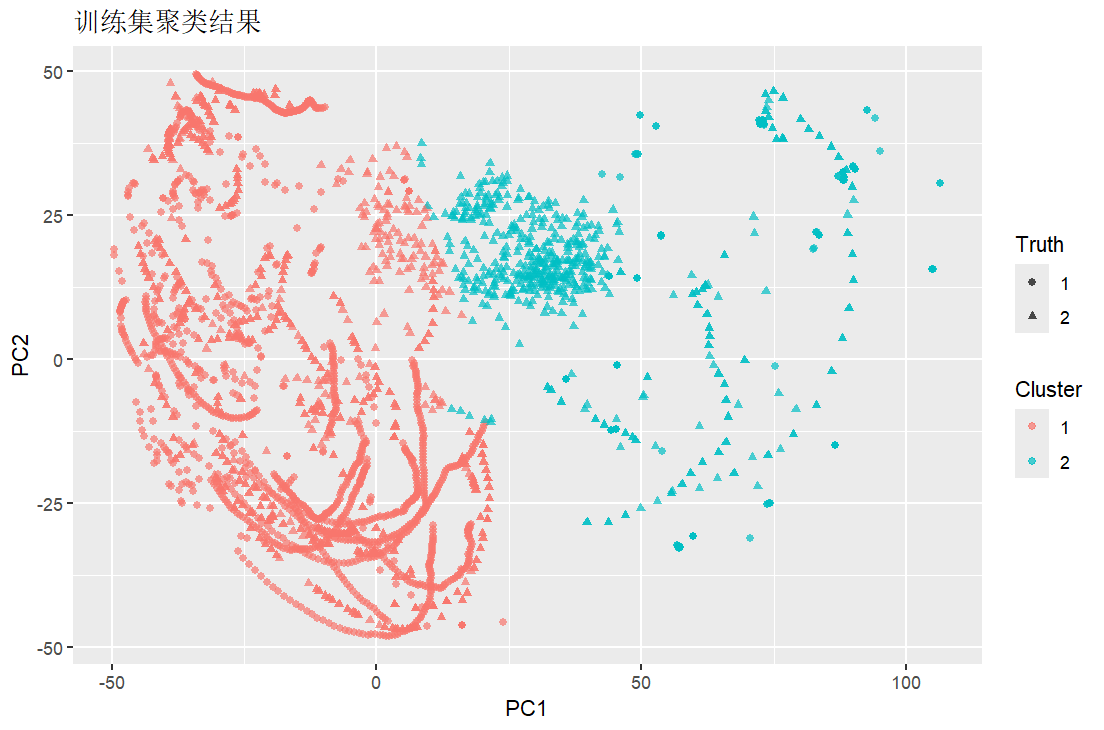
\includegraphics[width=0.5\linewidth]{imgs/cluster.png}
  \hspace{0.05\linewidth}
  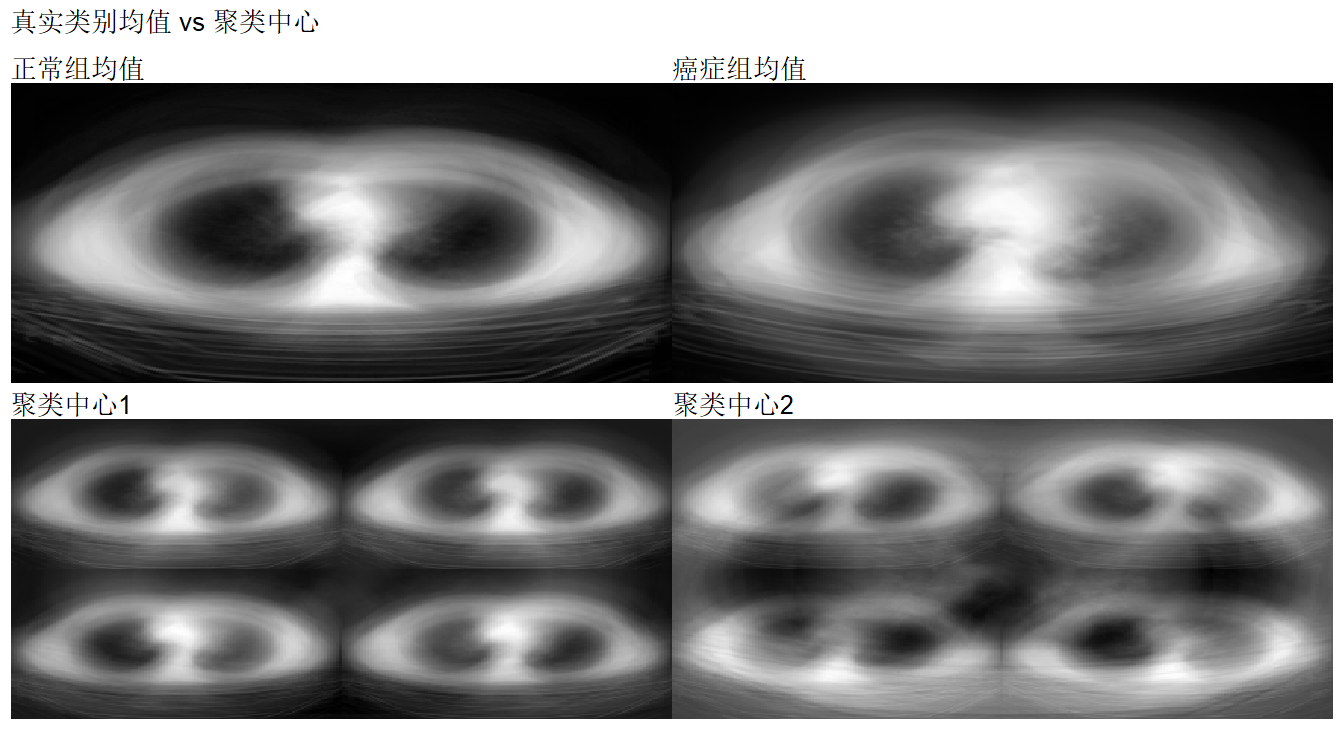
\includegraphics[width=0.5\linewidth]{imgs/cluster_compare.png}
  \caption{左图:前二主成分聚类图 CT 图;右图:聚类结果比较}
\end{figure}

\end{frame}


\section{二分类问题}

\begin{frame}{PCA + Logistic 回归}{}
\fontsize{9pt}{11pt}\selectfont

对于经过降维之后的数据向量 $x \in \mathbb{R}^q$ ,采用\textcolor{red}{Logistic 回归}的方式进行二分类,
标签为 normal 和 cancer ,从样本的 normal 和 cancer 中分别随机抽取 $1000$ 张图片,
总共 $2000$ 张图片进行训练,对于剩下的 $500$ 张 normal 和 $500$ 张 cancer 数据作为测试集,
用于检查模型的准确率。\\[0.5em]

对于 Logistic 回归模型,需要估计的参数为 $\beta \in \mathbb{R}^{q+1}$ ,记 $p = P(\text{cancer})$ 
为患癌概率,在原始数据 $X$ 的第一列前增加一列全 $1$ 向量 $\bf{1} \in \mathbb{R}^n$ ,
即有 $X = \left[\bf{1}\quad X \right]\in \mathbb{R}^{n\times (q+1)}$ ,于是有模型:

$$
\log \frac{p}{1-p} = X\cdot \beta
$$

使用数值方法估计参数 $\beta$ ,需要估计的参数量为 $q+1$ 个。

\end{frame}


\begin{frame}{PCA + Logistic 回归}{}
\fontsize{9pt}{11pt}\selectfont

模型参数的估计:对于已有的训练集 $T = \{ (x_1,\ y_1),\ (x_2,\ y_2),\ \cdots,\ (x_n,\ y_n) \}$ 
其中 $x_i \in \mathbb{R}^{q+1},\ y_i \in \{ 0,\ 1 \}$ 于是有:

$$
P(Y=1|x) = \pi(x) = \frac{\exp(x^T\beta)}{1+\exp(x^T\beta)}
$$

$$
P(Y=0|x) = 1-\pi(x) = 1-\frac{\exp(x^T\beta)}{1+\exp(x^T\beta)}
$$

通过极大化对数似然函数的方法,估计参数 $\beta$ :

$$
\max\limits_{\beta \in \mathbb{R}^{q+1}}\ L(\beta) = \sum\limits_{i=1}^n\ [ y_i\cdot \log \pi(x_i) + (1-y_i)\cdot \log (1- \pi(x_i) ]
$$

在本项目中,选择 $q = 10$ ,经过计算,得到结果。

\end{frame}


\begin{frame}{PCA + Logistic 回归}{}
\fontsize{9pt}{11pt}\selectfont
\begin{figure}
  \centering
  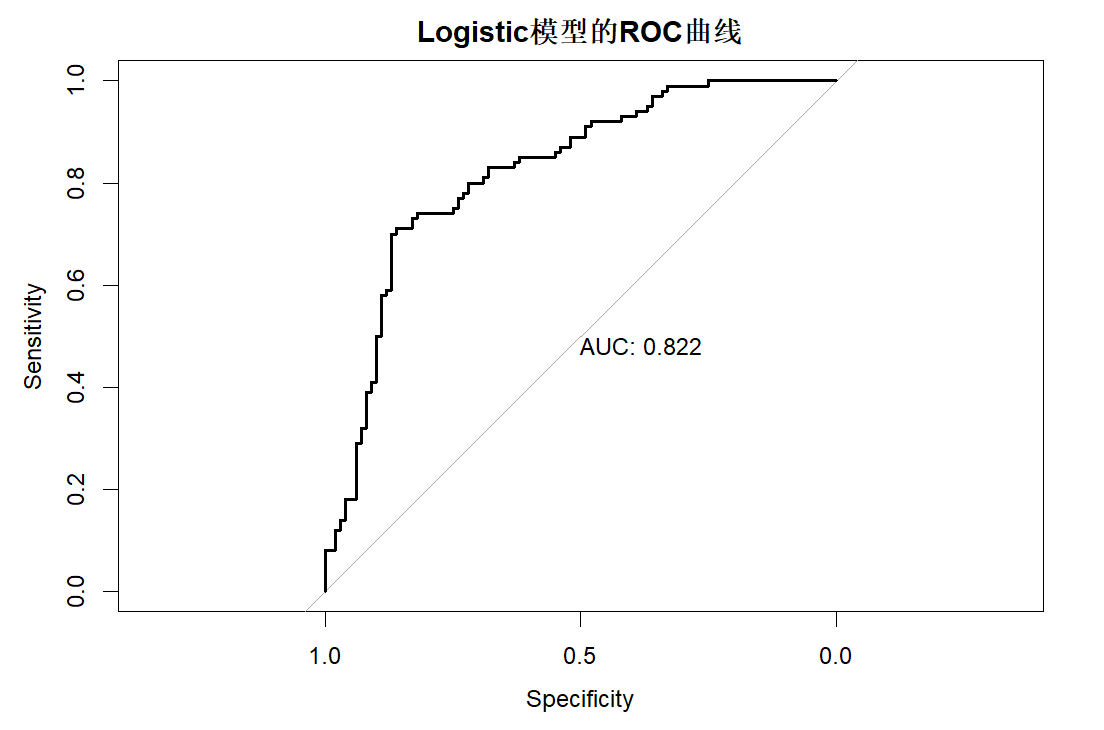
\includegraphics[width=0.45\linewidth]{imgs/roc.png}
  \hspace{0.05\linewidth}
  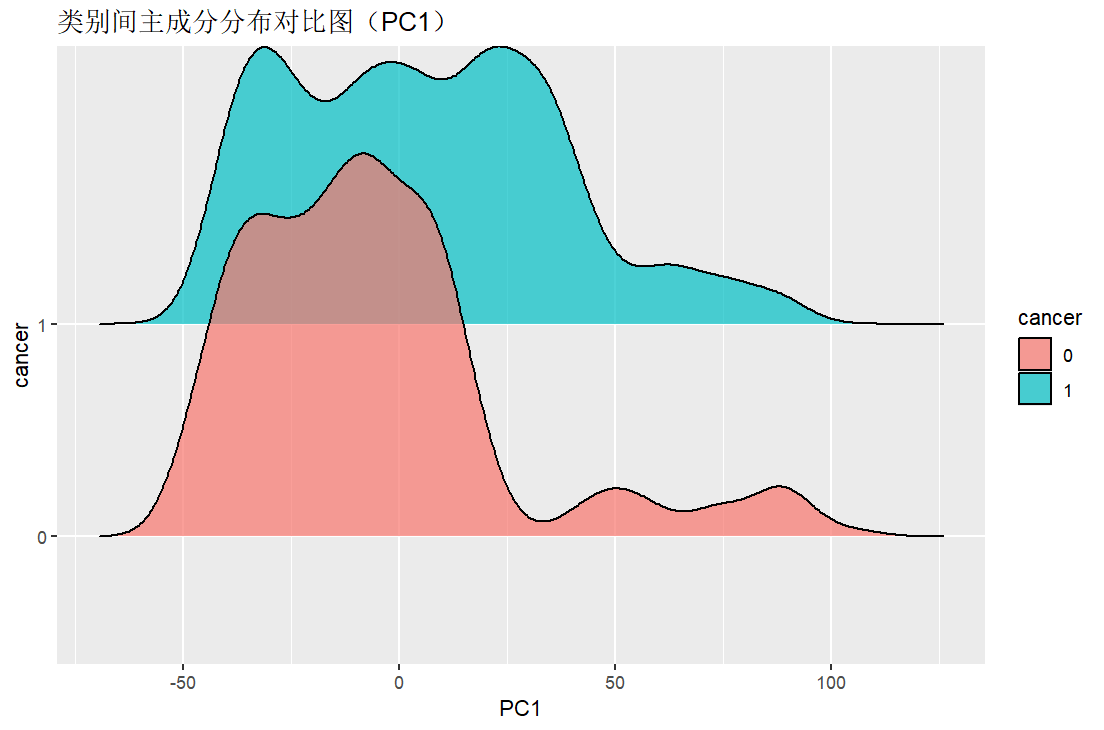
\includegraphics[width=0.45\linewidth]{imgs/pc1_compare.png}
  \caption{左图:Logistic ROC 曲线 CT 图;右图:类别主成分1分布图}
\end{figure}
\end{frame}

\begin{frame}{PCA + Logistic 回归}{}
\fontsize{9pt}{11pt}\selectfont

\lstinputlisting[language=R,caption=Result of Logistic]{resources/res.R}

\end{frame}

\begin{frame}{PCA + Logistic 回归}{}
\fontsize{9pt}{11pt}\selectfont

模型解释:对于变量/主成分 $PC_i$ ,每增加一个单位,患癌事件 cancer 的 odds 就会扩大/缩小 $e^{\beta_i}$ 倍。\\[0.5em]

测试集检查:在剩下的 $1000$ 张图片中进行预测,总体准确度达到了 $76.00\%$ ,混淆矩阵为

\lstinputlisting[language=R,caption=Result of Logistic]{resources/res2.R}

\end{frame}


\begin{frame}{PCA + Logistic 回归}{}
\fontsize{9pt}{11pt}\selectfont

\begin{figure}
    \centering
    \foreach \i in {1,...,5} {
        \begin{subfigure}[b]{0.18\textwidth}
            \includegraphics[width=\linewidth]{../PCA/pca\i.png}
            \caption*{主成分 \i}
        \end{subfigure}
    }

    \foreach \i in {6,...,10} {
        \begin{subfigure}[b]{0.18\textwidth}
            \includegraphics[width=\linewidth]{../PCA/pca\i.png}
            \caption*{主成分 \i}
        \end{subfigure}
    }
\end{figure}

\end{frame}


\begin{frame}{MaxPooling + Logistic + LASSO}{}
\fontsize{9pt}{11pt}\selectfont
直接使用 PCA ,若保留的主成分过多会带来计算复杂,若选取太少则会导致结果不佳。
所以,接下来我们采用 \textcolor{red}{Logistic + LASSO} 的方式进行间接变量选择。\\[0.5em]

LASSO 回归 (Robert Tibshirani 1996.\cite{tibshirani1996lasso}) :
在回归参数估计时,加入 L1 范数作为惩罚项。即对于本项目的 Logistic 回归的参数估计,需要优化的式子为:

$$
\min\limits_{\beta \in \mathbb{R}^{q'+1},\ \lambda \in \mathbb{R}^+}\ L(\beta) = -\frac{1}{n} \sum\limits_{i=1}^n\ [ y_i\cdot \log \pi(x_i) + (1-y_i)\cdot \log (1- \pi(x_i) ] + \lambda \| \beta \|_1
$$

其中 $\| \beta \|_1 = \sum_{j=1}^{q'+1} |\beta_j|$ 为向量 $\beta$ 的 L1 范数(若采用 L2 范
数,即 $\| \beta \|_2 = \sum_{j=1}^{q'+1} \beta^2_j$ ,则是岭回归 Ridge Regression)。
此时需要估计的参数数量为 $q'+1+1 = q'+2$ 。\\[0.5em]

先使用 MaxPooling 进行降维,故 $q' = 56 \times 56 = 3136$ ,于是本模型需要估计的参数数量为 $3138$ 个。\\[0.5em]

\end{frame}

\begin{frame}{MaxPooling + Logistic + LASSO}{}
\fontsize{9pt}{11pt}\selectfont

利用 R 语言自带的函数,增加 L1 范数作为惩罚项,得到 $\hat{\lambda}_{min} = 0.0022$ 。根据 LASSO 
回归选取的变量,我们构造特征图

\begin{figure}
  \centering
  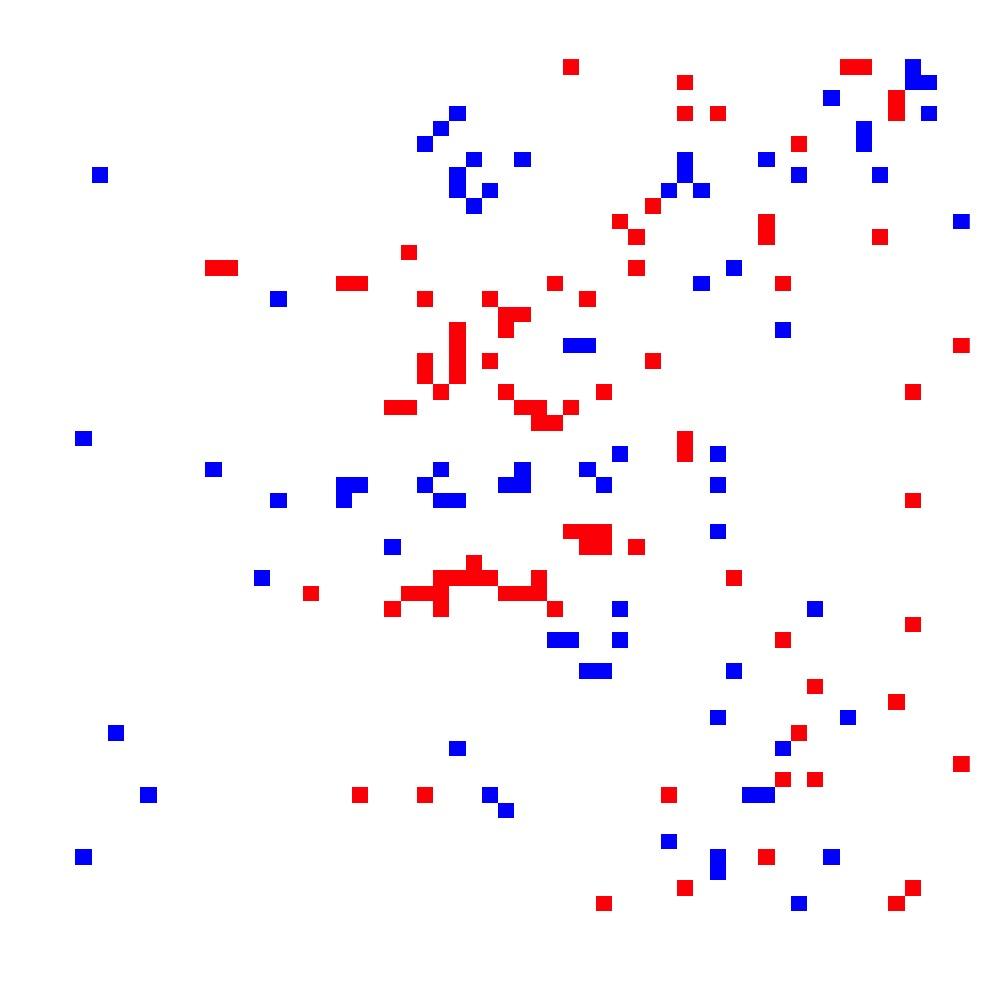
\includegraphics[width=0.5\textwidth]{../Features/lasso_features.jpg}
  \caption{红色代表“患癌点”,蓝色代表“正常点”}
\end{figure}

\end{frame}


\begin{frame}{MaxPooling + Logistic + LASSO}{}
\fontsize{9pt}{11pt}\selectfont
测试集检查:在剩下的 $1000$ 张图片中进行预测,总体准确度达到了 $98.3\%$,混淆矩阵为

\lstinputlisting[language=R,caption=Result of Logistic]{resources/res3.R}

\end{frame}

\section{拓展:卷积神经网络}

\begin{frame}{拓展:卷积神经网络}{}
\fontsize{9pt}{11pt}\selectfont
使用\textcolor{red}{卷积神经网络 CNN} 可以提高预测的准确率,
本项目实现了 2 个神经网络用于展示 ShallowCNNModel 和 CNNModel 。
其中 ShallowCNNModel 网络架构以及训练预测主程序框架来自 Kaggle 开源代码 
\href{https://www.kaggle.com/code/saikrishnakowshik/lung-ctscan}{lung-Ctscan}。
CNNModel 是本项目实现的更深的卷积神经,预测效果更好 (基于 AlexNet 网络框架) 。\\[0.5em]

模型在 Kaggle 提供的 GPU 环境下进行训练,最优结果如下所示。


\begin{table}
\centering
\caption{模型训练与测试表现}
\resizebox{\textwidth}{!}{ % 自动按页面宽度缩放
\begin{tabular}{lcccccc}
\toprule
Model & Train Loss & Train Acu (\%) & Val Loss & Val Acu (\%) & Test Loss & Test Acu (\%) \\
\midrule
\texttt{ShallowCNNModel} & 0.6076 & 94.52 & 0.1507 & 93.33 & 0.1240 & 94.89 \\
\texttt{CNNModel}        & 0.3526 & 97.52 & 0.1293 & 95.11 & 0.0835 & 96.67 \\
\bottomrule
\end{tabular}
}
\end{table}

可执行的 Notebook 代码已开源在 Kaggle ,
链接 \href{https://www.kaggle.com/code/iskage/ct-images-cnn/}{https://www.kaggle.com/code/iskage/ct-images-cnn/} ,
可使用 Kaggle 或 Colab 提供的 GPU 平台进行训练。(建议使用 GPU 加速训练,参数个数大约为 $57,012,034$ 即 $5700$ 万参数)

\end{frame}

\section{结论}

\begin{frame}{结论}{}
\fontsize{9pt}{11pt}\selectfont
本项目完成了对胸腔截面 CT 医学图像进行二分类的任务:
\begin{itemize}
  \item 使用主成分分析 (PCA) 和最大池化 (MaxPooling) 对图像进行特征提取和降维处理。
  \item 若采用简单的聚类分析,分类准确率为 $63.57\%$ 。
  \item 利用 Logistic 模型作为分类器,实现对数据集的二分类任务,最终测试集准确率达到 $76.00\%$ 。
  \item 为了在尽可能不损失信息和计算高效权衡,使用 MaxPooling 初步降维,然后使用 LASSO 回归辅助 Logistic 回归筛选变量,得到最终模型,测试集准确率高达 $98.30\%$ 。\\[1em]
\end{itemize}

\tiny{拓展:使用卷积神经网络进行分类,测试集准确率大约为 $94.22\%$ 到 $96.67\%$ 。}

\end{frame}


\begin{frame}[t]{参考文献}
  \tiny
  \bibliography{reference}
\end{frame}

\begin{frame}{Thanks Q\&A}
  \titlepage
\end{frame}


\end{document}